%%%%%%%%%%%%%%%%%%%%%%%%%%%%%%%%%%%%%%%%%%%%%%%%%%%%%%%%%%%%%%%%%%%%%%%%%%%%%%%
\section{Results}
\label{sec:results}
%%%%%%%%%%%%%%%%%%%%%%%%%%%%%%%%%%%%%%%%%%%%%%%%%%%%%%%%%%%%%%%%%%%%%%%%%%%%%%%

Both benchmarks were modeled with OpenMOC using MGXS generated by OpenMC for the null, degenerate and LNS spatial homogenization schemes. The eigenvalues and pin-wise fission and U-238 capture rates computed by OpenMOC are compared to the reference OpenMC solutions in \autoref{subsec:eigenvalues}, \autoref{subsec:fiss-rates} and \autoref{subsec:capt-rates}, respectively.


%%%%%%%%%%%%%%%%%%%%%%%%%%%%%%%%%%%%%%%%%%%%%%%%%%%%%%%%%%%%%%%%%%%%%%%%%%%%%%%
\subsection{Eigenvalues}
\label{subsec:eigenvalues}

The OpenMOC eigenvalues were compared to the reference OpenMC eigenvalues from \autoref{tab:keff-reference}. The eigenvalue bias $\Delta k$ was calculated by comparing the eigenvalue $k_{\textrm{eff}}^{\textrm{MOC}}$ from OpenMOC to the reference eigenvalue $k_{\textrm{eff}}^{\textrm{MC}}$ computed by OpenMC in units of per cent mille (pcm):

\begin{equation}
\label{eqn:delta-rho}
\Delta k = \left(k_{\textrm{eff}}^{\textrm{MOC}} - k_{\textrm{eff}}^{\textrm{MC}}\right) \times 10^{5}
\end{equation}

The bias is listed for both benchmarks and the three spatial homogenization schemes in \autoref{tab:keff-bias}. The slightly negative bias of a few hundred pcm is likely due to the flux separability approximation \citep{boyd2018sph}, which permits use of the scalar rather than the angular neutron flux to collapse cross sections. The eigenvalues for the three schemes are identical for the fuel assembly and are consistent to within 10 pcm for the colorset benchmark. As these results show, the choice of spatial homogenization scheme is inconsequential to the eigenvalue predictions. This is to be expected since the three methods use the same MC flux to collapse the MGXS and preserve global reactivity.

%It should be recalled that isotropic in lab scattering is used by OpenMC to compute both the reference solution and the MGXS. If anisotropic scattering were employed in OpenMC, one would expect quite different biases without a robust implementation of a higher order scattering kernel in OpenMOC.

\begin{table}[h!]
  \centering
  \caption{OpenMOC eigenvalue bias $\Delta k$.}
  \label{tab:keff-bias}
  \begin{tabular}{l c c c}
  \toprule
  \textbf{Benchmark} & \textbf{Null} & \textbf{Degenerate} & \textbf{LNS} \\
  \midrule
  Assembly & -161 & -161 & -161 \\
  Colorset & -142 & -132 & -138 \\
  \bottomrule
\end{tabular}
\end{table}


%%%%%%%%%%%%%%%%%%%%%%%%%%%%%%%%%%%%%%%%%%%%%%%%%%%%%%%%%%%%%%%%%%%%%%%%%%%%%%%
\subsection{Fission Rates}
\label{subsec:fiss-rates}

The OpenMOC energy-integrated pin-wise fission rates were compared to the reference OpenMC fission rates shown in \autoref{fig:fiss-assm} and \autoref{fig:fiss-reflector}. The percent relative errors for each pin's fission rates were computed and the maximum and mean errors are listed for both benchmarks and the three spatial homogenization schemes in \autoref{tab:fiss-errors}. In particular, the maximum errors are the maximum of the absolute values of the errors along with the appropriate sign, while the mean errors are the averages of the absolute error magnitudes.

\begin{table}[h!]
  \centering
  \caption{OpenMOC fission rate percent relative errors.}
  \label{tab:fiss-errors}
  \begin{tabular}{l l r r r}
  \toprule
  \textbf{Benchmark} & \textbf{Metric} & \textbf{Null} & \textbf{Degenerate} & \textbf{LNS} \\
  \midrule
  \multirow{2}{*}{Assembly} & Max  & 0.38 & 0.32 & 0.31 \\
                            & Mean & 0.07 & 0.08 & 0.08 \\
  \midrule
  \multirow{2}{*}{Colorset} & Max  & 0.76 & 0.60 & 0.71 \\
                            & Mean & 0.18 & 0.14 & 0.16 \\
  \bottomrule
\end{tabular}
\end{table}

The fission rate errors are only somewhat dependent on the spatial homogenization scheme used to compute MGXS in the fuel. In particular, the degenerate scheme reduces the max error by approximately 20\% compared to the null scheme. The max and mean errors for LNS homogenization are very nearly the same as those for degenerate homogenization for the assembly. Although the LNS errors for the colorset are reduced by approximately 10\% relative to null homogenization, they remain 15\% larger than those for the degenerate scheme. This is due to the fact that LNS homogenizes the MGXS of fuel pins along the assembly-reflector interface with those at the inter-assembly interfaces, rather than distinguishing them into separate groupings of pins to account for the additional moderation provided by the reflector.

The spatial distributions of fission rate errors are plotted as heatmaps for each benchmark in \autoref{fig:assm-fiss-errors} and \autoref{fig:reflector-fiss-errors}. In the assembly benchmark, the fission rates are generally overpredicted for pins inside the outermost ring of CRGTs, and overpredicted for the four pins diagonally adjacent to the central instrument tube and facially adjacent to the outermost rings of CRGTs. In the case of the colorset benchmark, the fission rates are overpredicted for pins along the assembly-reflector interface and underpredicted for the most interior pins along the bottom-right assembly's inter-assembly interfaces.

Although the heatmaps illustrate systematic trends in the pin-wise fission errors, the errors maintain a highly similar structure for all three spatial homogenization schemes. This indicates that the fission rate errors are only marginally impacted by inter-pin spatial self-shielding\footnote{This may not remain true for coarser energy group structures than the 70-group structure used in this paper.}, and are instead driven by the energy, angle and spatial discretization used in the deterministic multi-group calculation.

%For the PWR benchmarks modeled here, the moderation provided by neighboring CRGTs and reflectors softens the flux for nearby fuel pins and should be modeled when collapsing pin-wise MGXS for high-fidelity multi-group transport calculations.

\clearpage

\begin{figure}[H]
  \centering 
\begin{subfigure}{0.45\textwidth}
  \centering
  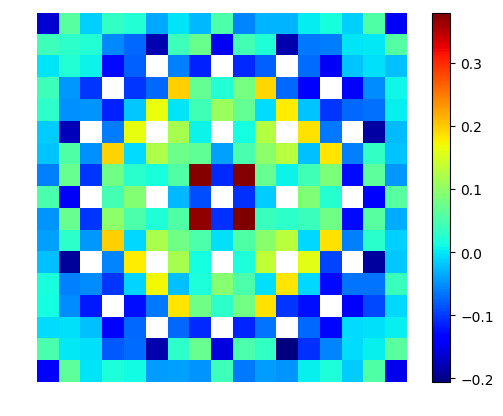
\includegraphics[width=\linewidth]{figures/assembly/fiss-null-errors}
  \caption{}
  \label{fig:assm-fiss-null-error}
\end{subfigure}
\begin{subfigure}{0.45\textwidth}
  \centering
  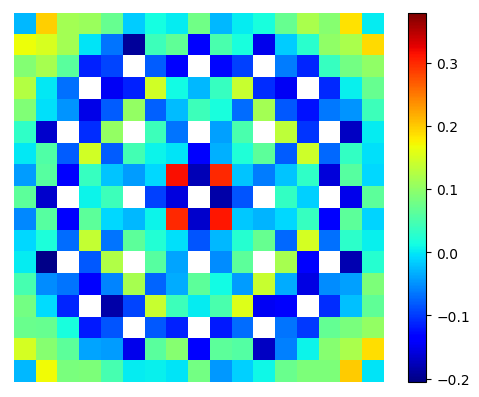
\includegraphics[width=\linewidth]{figures/assembly/fiss-degenerate-errors}
  \caption{}
  \label{fig:assm-fiss-degen-error}
\end{subfigure}
\begin{subfigure}{0.45\textwidth}
  \centering
  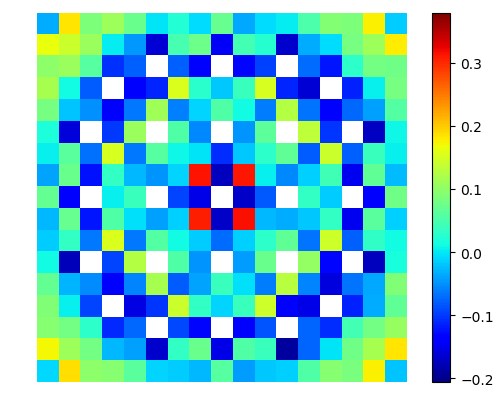
\includegraphics[width=\linewidth]{figures/assembly/fiss-lns-errors}
  \caption{}
  \label{fig:assm-fiss-lns-error}
\end{subfigure}
\caption{OpenMOC fission rate percent relative errors for the assembly with null (a), degenerate (b) and LNS (c) spatial homogenization.}
\label{fig:assm-fiss-errors}
\end{figure}

\begin{figure}[H]
  \centering 
\begin{subfigure}{0.45\textwidth}
  \centering
  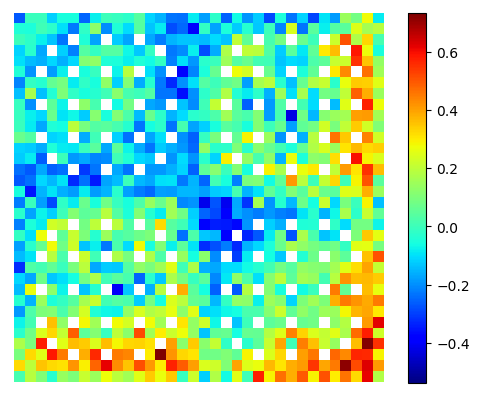
\includegraphics[width=\linewidth]{figures/reflector/fiss-null-errors}
  \caption{}
  \label{fig:reflector-fiss-null-error}
\end{subfigure}
\begin{subfigure}{0.45\textwidth}
  \centering
  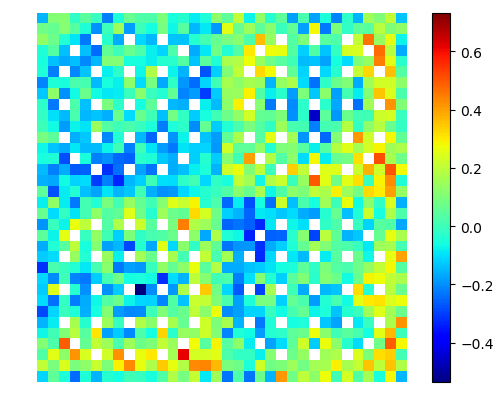
\includegraphics[width=\linewidth]{figures/reflector/fiss-degenerate-errors}
  \caption{}
  \label{fig:reflector-fiss-degen-error}
\end{subfigure}
\begin{subfigure}{0.45\textwidth}
  \centering
  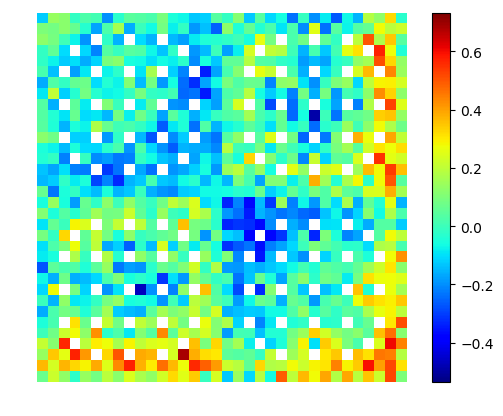
\includegraphics[width=\linewidth]{figures/reflector/fiss-lns-errors}
  \caption{}
  \label{fig:reflector-fiss-lns-error}
\end{subfigure}
\caption{OpenMOC fission rate percent relative errors for the colorset with null (a), degenerate (b) and LNS (c) spatial homogenization.}
\label{fig:reflector-fiss-errors}
\end{figure}


%%%%%%%%%%%%%%%%%%%%%%%%%%%%%%%%%%%%%%%%%%%%%%%%%%%%%%%%%%%%%%%%%%%%%%%%%%%%%%%
\subsection{Capture Rates}
\label{subsec:capt-rates}

The OpenMOC energy-integrated pin-wise U-238 capture rates were compared to the reference OpenMC capture rates shown in \autoref{fig:capt-assm} and \autoref{fig:capt-reflector} for the assembly and reflector, respectively. The percent relative errors for each pin's capture rates were computed and the maximum and mean errors are listed for both benchmarks and the three spatial homogenization schemes in \autoref{tab:capt-errors}. In particular, the maximum errors are the maximum of the absolute values of the errors along with the appropriate sign, while the mean errors are the averages of the absolute error magnitudes.

\begin{table}[h!]
  \centering
  \caption{OpenMOC U-238 capture rate percent relative errors.}
  \label{tab:capt-errors} 
  \begin{tabular}{l l r r r}
  \toprule
  \textbf{Benchmark} & \textbf{Metric} & \textbf{Null} & \textbf{Degenerate} & \textbf{LNS} \\
  \midrule
  \multirow{2}{*}{Assembly} & Max  & -1.101 &  0.386 & 0.290 \\
                            & Mean &  0.479 &  0.086 & 0.076 \\
  \midrule
  \multirow{2}{*}{Colorset} & Max  & -1.969 & -0.783 & -1.964 \\
                            & Mean &  0.478 &  0.165 & 0.236 \\
  \bottomrule
\end{tabular}
\end{table}

The capture rate errors are more dependent on the spatial homogenization scheme used to compute MGXS in the fuel than are the fission rate errors. In particular, the degenerate scheme produces much smaller maximum and mean errors than the null scheme. The maximum error is greater than 1\% for both benchmarks with the null scheme, but is reduced by 2 -- 5$\times$ with the use of degenerate homogenization. This underscores the importance of accounting for spatial heterogeneities when generating MGXS to predict U-238 capture and subsequently Pu-239 production in LWRs. The moderation provided by neighboring CRGTs and reflectors softens the flux for nearby fuel pins and should be modeled when collapsing pin-wise MGXS for high-fidelity multi-group transport calculations.

The max and mean U-238 capture rate errors are reduced by 3.7$\times$ and 6.3$\times$, respectively, for LNS with respect to null homogenization for the assembly. This demonstrates that LNS homogenization more accurately models inter-pin spatial self-shielding effects in pin-wise MGXS than null homogenization. Furthermore, the max and mean errors are reduced by 10\% and 25\% relative to degenerate homogenization. This latter observation indicates that LNS reduces the statistical uncertainties of the MC-generated MGXS by averaging the MGXS for each grouping of fuel pins, resulting in MGXS with smaller uncertainties than those generated by degenerate homogenization. However, the results are significantly different for the colorset. In particular, the max error for the colorset with LNS homogenization is very nearly the same as those for null homogenization. The MGXS for the fuel pins near the assembly-reflector interface are not separately homogenized with LNS and thus fail to account for the additional moderation from the reflector.

The spatial distributions of capture rate errors are plotted as heatmaps for the assembly and colorset in \autoref{fig:assm-capt-errors} and \autoref{fig:reflector-capt-errors}, respectively. The null scheme exhibits the largest errors for pins near CRGTs and along the inter-assembly and assembly-reflector interfaces, while the degenerate scheme produces a much more even error distribution across the pins in the colorset. The heatmaps illustrate similar error distributions for degenerate and LNS spatial homogenization for the assembly, but systematic deviations for the colorset. The LNS scheme smooths the error distribution, but exhibits large errors for the single outermost row of pins adjacent to the reflector, and to a lesser extent, the pins along the inter-assembly interfaces. More specifically, the U-238 capture rates are under-predicted near the reflector and over-predicted for interior pins.

This result is indicative of the collective homogenization of all pins along the exterior of each assembly irregardless of the neighboring spatial zones. The flux at U-238 capture resonance energies is more shielded for pins adjacent to the reflector than for interior pins, resulting in larger U-238 capture MGXS. LNS homogenizes the larger MGXS for pins along the reflector with the smaller capture MGXS for interior pins, which leads to a systematic under-prediction for the outermost pins. Nevertheless, flux-weighted spatial homogenization ensures that the errors improve the most for the interior pins with the largest reaction rates (see \autoref{fig:fiss-capt-rates}).

\clearpage

\begin{figure}[H]
  \centering 
\begin{subfigure}{0.45\textwidth}
  \centering
  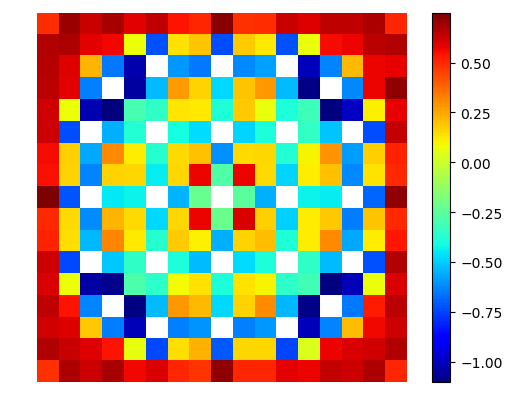
\includegraphics[width=\linewidth]{figures/assembly/capt-null-errors}
  \caption{}
  \label{fig:assm-capt-null-error}
\end{subfigure}
\begin{subfigure}{0.45\textwidth}
  \centering
  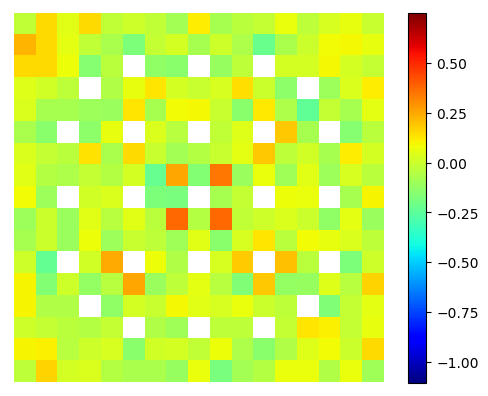
\includegraphics[width=\linewidth]{figures/assembly/capt-degenerate-errors}
  \caption{}
  \label{fig:assm-capt-degen-error}
\end{subfigure}
\begin{subfigure}{0.45\textwidth}
  \centering
  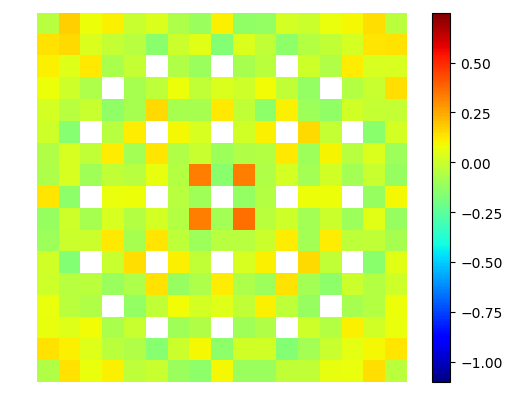
\includegraphics[width=\linewidth]{figures/assembly/capt-lns-errors}
  \caption{}
  \label{fig:assm-capt-lns-error}
\end{subfigure}
\caption{OpenMOC U-238 capture rate percent relative errors for the assembly with null (a), degenerate (b) and LNS (c) spatial homogenization.}
\label{fig:assm-capt-errors}
\end{figure}

\begin{figure}[H]
  \centering 
\begin{subfigure}{0.45\textwidth}
  \centering
  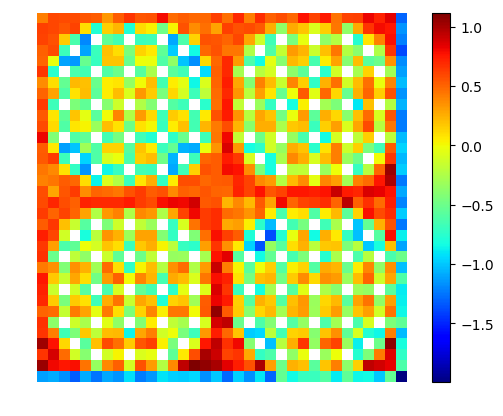
\includegraphics[width=\linewidth]{figures/reflector/capt-null-errors}
  \caption{}
  \label{fig:reflector-capt-null-error}
\end{subfigure}
\begin{subfigure}{0.45\textwidth}
  \centering
  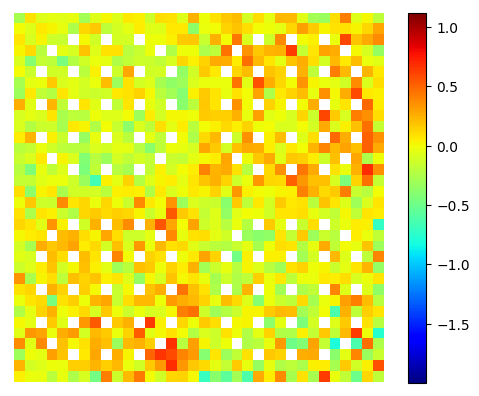
\includegraphics[width=\linewidth]{figures/reflector/capt-degenerate-errors}
  \caption{}
  \label{fig:reflector-capt-degen-error}
\end{subfigure}
\begin{subfigure}{0.45\textwidth}
  \centering
  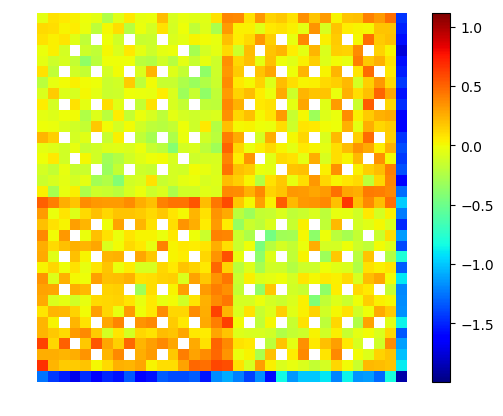
\includegraphics[width=\linewidth]{figures/reflector/capt-lns-errors}
  \caption{}
  \label{fig:reflector-capt-lns-error}
\end{subfigure}
\caption{OpenMOC U-238 capture rate percent relative errors for the colorset with null (a), degenerate (b) and LNS (c) spatial homogenization.}
\label{fig:reflector-capt-errors}
\end{figure}
